
Because $x$ and the longitudinal spatial separation $b \cdot P$ are Fourier conjugate variables, mapping the $x$-dependence requires a Fourier transform of these amplitudes with respect to $b \cdot P$. Analytically, the $x$-dependent Sivers shift takes the form:
\begin{widetext}
\begin{align}
   \langle \vect{k}_y \rangle_{TU}(\vprp{\bvec}^2,x,\zetahat,\eta v \tcdot P) 
	&\ \equiv\ \mN \frac{\tilde f_{1T}^{\perp(1)}(\vprp{\bvec}^2,x;\zetahat,\ldots,\eta v \tcdot P)}{\tilde f_1^{(0)}(\vprp{\bvec}^2,x;\zetahat,\ldots,\eta v \tcdot P)}  \\
 &=-m_{N} \frac{\int d(b\cdot P)e^{ix(b\cdot P)} \tAmp_{12B}(\bvec^2,\bvec \tcdot P,(\bvec \tcdot P) R(\zetahat^2)/\mN^2,-1/(\mN\zetahat)^2,\eta v \tcdot P)}{\int d(b\cdot P)e^{ix(b\cdot P)}\tAmp_{2B}(\bvec^2,\bvec \tcdot P,(\bvec \tcdot P) R(\zetahat^2)/\mN^2,-1/(\mN\zetahat)^2,\eta v \tcdot P)}  \\
 &=-m_{N} \frac{\int d(b\cdot P)e^{ix(b\cdot P)} \left[\tAmp_{12B}^{\text{Re}}(\cdots)+i\tAmp_{12B}^{\text{Im}}(\cdots)\right]}{\int d(b\cdot P)e^{ix(b\cdot P)}\left[\tAmp_{2B}^{\text{Re}}(\cdots)+i\tAmp_{2B}^{\text{Im}}(\cdots)\right]}\\
 &=-m_{N} \frac{\int d(b\cdot P)\left[\cos{\left(x(b\cdot P)\right)}+i\sin{\left(x(b\cdot P)\right)}\right] \left[\tAmp_{12B}^{\text{Re}}(\cdots)+i\tAmp_{12B}^{\text{Im}}(\cdots)\right]}{\int d(b\cdot P)\left[\cos{\left(x(b\cdot P)\right)}+i\sin{\left(x(b\cdot P)\right)}\right]\left[\tAmp_{2B}^{\text{Re}}(\cdots)+i\tAmp_{2B}^{\text{Im}}(\cdots)\right]}\\
 &=-m_{N} \frac{\int d(b\cdot P) \left[\cos{\left(x(b\cdot P)\right)}\tAmp_{12B}^{\text{Re}}(\cdots)-\sin{\left(x(b\cdot P)\right)}\tAmp_{12B}^{\text{Im}}(\cdots)\right]}{\int d(b\cdot P)\left[\cos{\left(x(b\cdot P)\right)}\tAmp_{2B}^{\text{Re}}(\cdots)-\sin{\left(x(b\cdot P)\right)}\tAmp_{2B}^{\text{Im}}(\cdots)\right]} \\
 &=-m_{N} \frac{\left[\tAmp_{12B}^{[x]\text{Re}}(b^2,x,\zetahat,\eta v \tcdot P)-\tAmp_{12B}^{[x]\text{Im}}(b^2,x,\zetahat,\eta v \tcdot P)\right]}{\left[\tAmp_{2B}^{[x]\text{Re}}(b^2,x,\zetahat,\eta v \tcdot P)-\tAmp_{2B}^{[x]\text{Im}}(b^2,x,\zetahat,\eta v \tcdot P)\right]}
 \label{eq:sivers_shift_xdep}
 \end{align}
\end{widetext}
 Expanding the Fourier phase factor into its trigonometric components isolates the real and imaginary contributions of the amplitudes to the Sivers shift. Because the integration over $d(b \cdot P)$ is performed over a symmetric domain, the non-vanishing terms of the integral are dictated by the parity of the integrands with respect to $b \cdot P$. The trigonometric weights $\cos\left(x(b\cdot P)\right)$ and $\sin\left(x(b\cdot P)\right)$ are even and odd, respectively.

This harmonic symmetry filters the invariant amplitudes based on their behavior under Hermitian conjugation. By Eqs.~\eqref{conditi_hermitian} and~\eqref{eq-ReIm-parity}, the real components $\tAmp_{2B}^{\text{Re}}$ and $\tAmp_{12B}^{\text{Re}}$ are even functions of $b \cdot P$, while the imaginary components $\tAmp_{2B}^{\text{Im}}$ and $\tAmp_{12B}^{\text{Im}}$ are odd. (Parity in $b$ is parity in $b\cdot P$ here, because $\bvec^2$ is unchanged under $b\to-b$, $v\cdot b$ is tied to $b\cdot P$ by Eq.~\eqref{eq-lindeprel}, and $R(\zetahat^2)$ is real.) Only the symmetric products therefore survive the integration, i.e., the even real amplitudes coupled with the cosine term and the odd imaginary amplitudes coupled with the sine term. Here, $\tAmp_{iB}^{[x]\text{Re}}$ and $\tAmp_{iB}^{[x]\text{Im}}$ are the Fourier-transformed amplitudes. Note that, since $\tAmp_{iB}^{\text{Im}}$ is odd in $(P\cdot b)$, its Fourier transform gives an imaginary solution, i. e. $\int \frac{d(\bvec \tcdot P)}{2\pi}e^{ix(b\cdot P)}\tAmp_{iB}^{\text{Im}}=i\tAmp_{iB}^{[x]\text{Im}}$, this results in
\begin{align}
    \int \frac{d(\bvec \tcdot P)}{2\pi}e^{ix(b\cdot P)} \left[\tAmp_{iB}^{\text{Re}}+i\tAmp_{iB}^{\text{Im}}\right]=&\left[\tAmp_{iB}^{[x]\text{Re}}+i^2\tAmp_{iB}^{[x]\text{Im}}\right]\\
    =&\left[\tAmp_{iB}^{[x]\text{Re}}-\tAmp_{iB}^{[x]\text{Im}}\right]
    \label{reminusimag-amp}
\end{align}
for both unpolarized and Sivers TMD amplitudes. 

The parity components are extracted from the lattice data as described in Secs.~\ref{sec:b_separation_paths} and~\ref{sec:solving_amplitudes}.


\subsection{Collins-Soper parameter on the lattice}
\label{sec:collins_soper_parameter}
The Collins-Soper parameter $\hat{\zeta}$ of Eq.~\eqref{eq-zeta} is
\begin{equation}
	\hat \zeta \equiv \zeta / 2 \mN =  \frac{v \cdot P}{\sqrt{|v^2|} \sqrt{P^2}}.
	\label{eq-zeta-again}
\end{equation}

On the lattice, the staple direction $v$ must be space-like ($v^2 < 0$), so the physical TMD limit is recovered only by extrapolating $\hat{\zeta} \to \infty$. In practice, since $v$ is a purely spatial vector on the lattice ($v_0 = 0$), increasing $\hat{\zeta}$ requires simulating the nucleon at progressively higher spatial momenta $\vect{P}$. Tracking the evolution of the Sivers shift across multiple $\hat{\zeta}$ values is therefore necessary for phenomenological predictions.

\subsection{Kinematic constraints for scanning the full range of $b\cdot P$}
\label{sec:kinematic_constraints}
We now move to the frame in which the lattice calculation is performed. To perform the Fourier transform over $b \cdot P$, we require a lattice geometry with both non-zero $b \cdot P$ and zero $b \cdot P$. However, the Lorentz-invariant arguments of the amplitudes are not independent. The phenomenological frame ($b^+=0, \vprp{P}=0$) enforces the constraint of Eq.~\eqref{eq-lindeprel}. Expanding the dot products in the case where the momentum is directed along the 1-axis ($P = (E, P_1, 0, 0)$), we find:
\begin{align}
    b_{1}|v|\left[\frac{P_{1}}{m_{N}}\left(\hat{\zeta}-\sqrt{\hat{\zeta}^2+1}\right)+\hat{\zeta}\frac{m_{N}}{P_{1}}\right]=\vec{v}_{T}\cdot\vec{b}_{T} \ .\label{constraints}
\end{align}
To satisfy this equation over a continuous range of $b \cdot P$ without coupling the transverse separation $\vec{b}_T$ directly to the longitudinal staple geometry, we orient the transverse separation vectors orthogonally. By choosing $\vec{v}_{T}=(0,v_{3})$ and $\vec{b}_{T}=(b_{2},0)$, the right-hand side identically vanishes ($\vec{v}_{T}\cdot\vec{b}_{T} = 0$). This is not the only choice, but it is convenient for a lattice calculation because both $b$ and $v$ can remain in 2-dimensional lattice planes. In general, $b$ and $v$ may have to point in arbitrary directions in three-dimensional space.

For a given lattice momentum, setting the bracket to zero fixes $\hat\zeta$ and the staple direction; the explicit calculation for the lowest momentum $P_1=-1$ is in Appendix~\ref{app:explicit_zeta}. The results for all four momenta are collected in Table~\ref{tab:zeta_directions}.


\subsection{Lattice parameter space}
\label{sec:lattice_parameter_space}
This geometric calculation is repeated over a range of nucleon momenta to increase $\hat{\zeta}$ systematically. The resulting constraint parameters are summarized in Table \ref{tab:zeta_directions}.

\begin{table}[htbp]
    \centering
    \renewcommand{\arraystretch}{1.3}
    \begin{tabular}{|c|c|c|}
    \hline
        $\vect{P}\cdot a\hat{L}/(2\pi)$ & $\hat{\zeta}$ &  $v_{1}$\\
        \hline
        $(-1,0,0)$ & $\pm 0.090772$ &$v_{1}=\pm 0.301~v_{3}$\\
        \hline
        $(-2,0,0)$ & $\pm 0.294367$ &$v_{1}=\pm 0.531~v_{3}$\\
        \hline
        $(-3,0,0)$ & $\pm 0.539684$ &$v_{1}=\pm 0.689~v_{3}$\\
        \hline
        $(-4,0,0)$ & $\pm 0.785756$ &$v_{1}=\pm 0.786~v_{3}$\\
        \hline
    \end{tabular}
    \caption{Resulting Collins-Soper parameters ($\hat{\zeta}$) and the necessary geometric constraint on the staple vector components to ensure the full $b \cdot P$ range is scanned.}
    \label{tab:zeta_directions}
\end{table}

\begin{table}[htbp]
    \centering
    \renewcommand{\arraystretch}{1.3}
    \resizebox{\columnwidth}{!}{\begin{tabular}{|c|c|c|}
    \hline
       $\vect{\bvec}/a$  &  $\eta \vect{v}/a$ & $\vect{P}\cdot a\hat{L}/(2\pi)$\\
       \hline
        $(b_{1},b_{2},0)$ & $ \eta\cdot(v_{1},0,v_{3})$, $\eta=0,\cdots,10$  & $(n,0,0)$, $n=-1,-2,-3,-4$\\
        \hline
    \end{tabular}}
    \caption{Configuration parameters for the Lattice QCD non-local matrix element extraction. Our lattice size is $\{\hat{L}^3\times\hat{T}\}=\{32^3\times96\}$ and the lattice spacing is $a=0.11403\text{ fm}$.}
    \label{tab:lattice_params}
\end{table}
A consequence of Table \ref{tab:zeta_directions} is that the staple vector $v$ cannot align cleanly with the Cartesian axes of the Euclidean grid. Instead, it must point in an off-axis direction within the $v_1-v_3$ plane. For example, to achieve $v_1 = 0.301~v_3$ at $|P| = 1$, the Wilson line must trace an oblique, step-wise path across the discrete lattice sites (e.g., traversing roughly three lattice spacings in the 1-direction for every ten in the 3-direction). Figure \ref{fig:v_allzetahat} plots the resulting staple directions in the $v_1-v_3$ plane for all four Collins-Soper values in Table \ref{tab:zeta_directions}.

\begin{figure}[htpb]
    \centering
    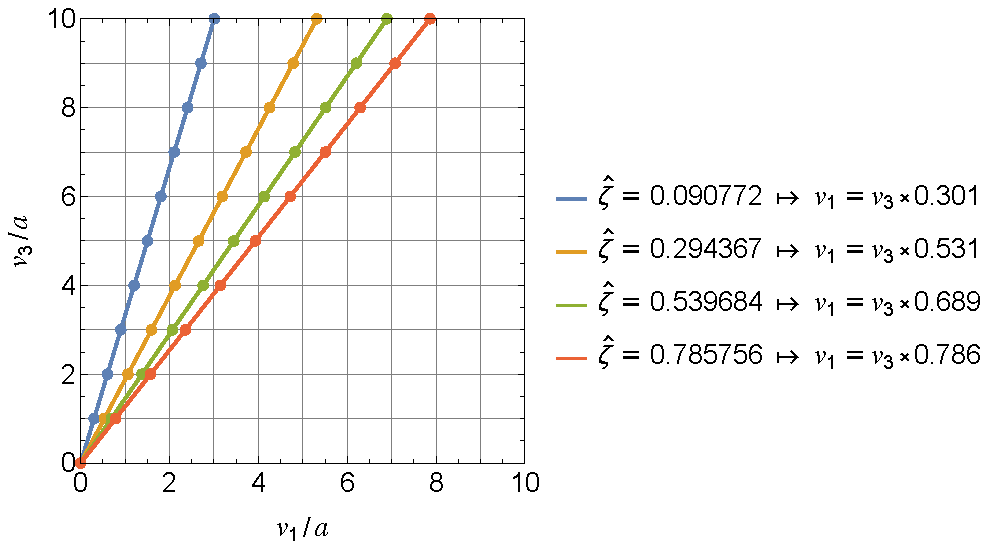
\includegraphics[width=0.7\linewidth]{figures/v1_v2_allzetahat_plot.pdf}
    \caption{Directions of the spatial staple vectors $\vect{v}$ mapped in the $v_1-v_3$ plane. Each vector corresponds to the requisite geometry to satisfy the $b \cdot P \neq 0$ constraint for the four sequential Collins-Soper parameters $\hat{\zeta}$.}
    \label{fig:v_allzetahat}
\end{figure}

\subsection{Off-axis staples and interpolation}
\label{sec:offaxis_v}
\label{sec:spatial_interpolation}
To evaluate the correlation function as a function of the staple extent, we scale the direction vector $\vect{v}$ by an increment $\eta$, and $\vect{v}$ is a unit vector. The physical length of the staple is thus governed by the coordinate $\eta \vect{v}/a$. Because $\vect{v}$ points in a continuous, off-axis direction, scaling it by integer values of $\eta$ generally yields target coordinates that fall somewhere between the discrete Cartesian lattice sites. 

 To access the continuous off-axis coordinate $\eta \vect{v}/a$, we employ a spatial bounding and interpolation strategy. Rather than constructing a single, potentially biased step-wise path (a ``staircase'') that roughly approximates the vector, we compute the observable at multiple distinct integer lattice sites surrounding the exact ideal target coordinate. We reach these bounding coordinates through specific permutations of unit links. A path sequence denoted $\{1,3,1\}$ is a single link in the $\hat{x_{1}}$ direction, followed by one in the $\hat{x_{3}}$ direction and a final link in the $\hat{x_{1}}$ direction, which lands at the integer coordinate $(2,0,1)$. By varying these step sequences, we gather data at three to four adjacent lattice sites (e.g., on either side of the target along the $x^3$ slice). 

Once these bounding matrix elements are computed, we perform a spatial interpolation inside the Jackknife resampling loop to extract the value at the continuous target coordinate $\eta \vect{v}/a$. The interpolation reduces discretization artifacts and the staircase errors of off-axis Wilson lines; the procedure is described below. Figures \ref{fig:v_path_P-1}--\ref{fig:v_path_P-4} and Tables \ref{tab:eta_table_P-1}--\ref{tab:eta_table_P-4} of Appendix~\ref{app:paths} show the ideal continuous trajectories for each nucleon momentum, together with the corresponding discrete bounding paths and link sequences.
Before interpolating to the off-axis target $\eta \vect{v}/a$, we must account for path degeneracy. Because the lattice gauge links are restricted to the Cartesian axes, there are multiple step-wise permutations (different side-link paths) that terminate at the same physical lattice coordinate. While these paths are geometrically equivalent at their endpoints, they are different lattice operators with the same continuum limit and can have distinct discretization artifacts and gauge noise. As illustrated in Figure \ref{fig:example_2path}, to improve the symmetry, we average the correlation functions evaluated over all degenerate paths that share the same endpoint. Path averaging symmetry-improves the lattice operators and reduces the gauge noise before any interpolation. % TODO(Hari): quantify the noise reduction; state that the same path set is used for every $\Gamma$

\begin{figure}[htpb]
    \centering
    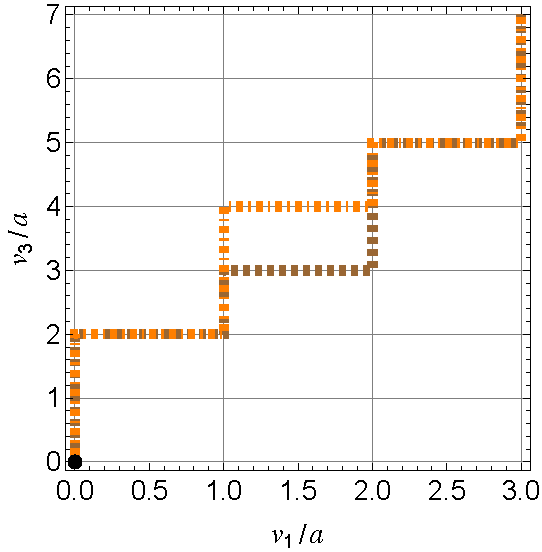
\includegraphics[width=0.5\linewidth]{figures/Example_v_plot_with_2path.pdf}
    \caption{Illustration of path degeneracy. Two distinct step-wise gauge link permutations (e.g., solid and dashed lines) terminate at the identical discrete lattice coordinate. We average the correlators from these equivalent paths to suppress local gauge noise before interpolation.}
    \label{fig:example_2path}
\end{figure}

Once we obtain the symmetry-improved (path-averaged) correlators at the discrete bounding sites, we perform a 1-dimensional interpolation. For a fixed transverse staple extent $v_3$, the kinematic constraint dictates an ideal continuous longitudinal component, $v_1^{\text{constraint}}$. The surrounding discrete lattice sites provide correlators at actual simulated coordinates, $v_1^{\text{lattice}}$. We define the fractional deviation from the ideal path as:
\begin{equation}
    \Delta v_1 = \frac{v_1^{\text{constraint}} - v_1^{\text{lattice}}}{a} \ .
\end{equation}
By calculating the observable at three or more bounding lattice sites, we generate a set of data points as a function of this deviation $\Delta v_1$. Within each Jackknife resampling bin (to preserve the covariance and statistical error), we perform a quadratic interpolation over these points. We then extract the physical amplitude on the continuous constraint trajectory by evaluating the interpolating polynomial exactly at $\Delta v_1 = 0$. 


A representative example of this interpolation procedure is shown in Figure \ref{fig:interpolation_ex} for a specific staple extent ($\eta=7$) and nucleon momentum ($P_1 = -1$). The red data points represent the path-averaged lattice evaluations at the discrete bounding sites, plotted against their deviation from the ideal trajectory. The solid gray curve denotes the quadratic interpolation, and the blue point highlights the final extracted physical value at $\Delta v_1 = 0$. We apply this procedure to all Dirac structures ($\Gamma$), separately for the real ($b\cdot P$-even) and imaginary ($b\cdot P$-odd) parts of the amplitudes.

\begin{figure}[htpb]
    \centering
    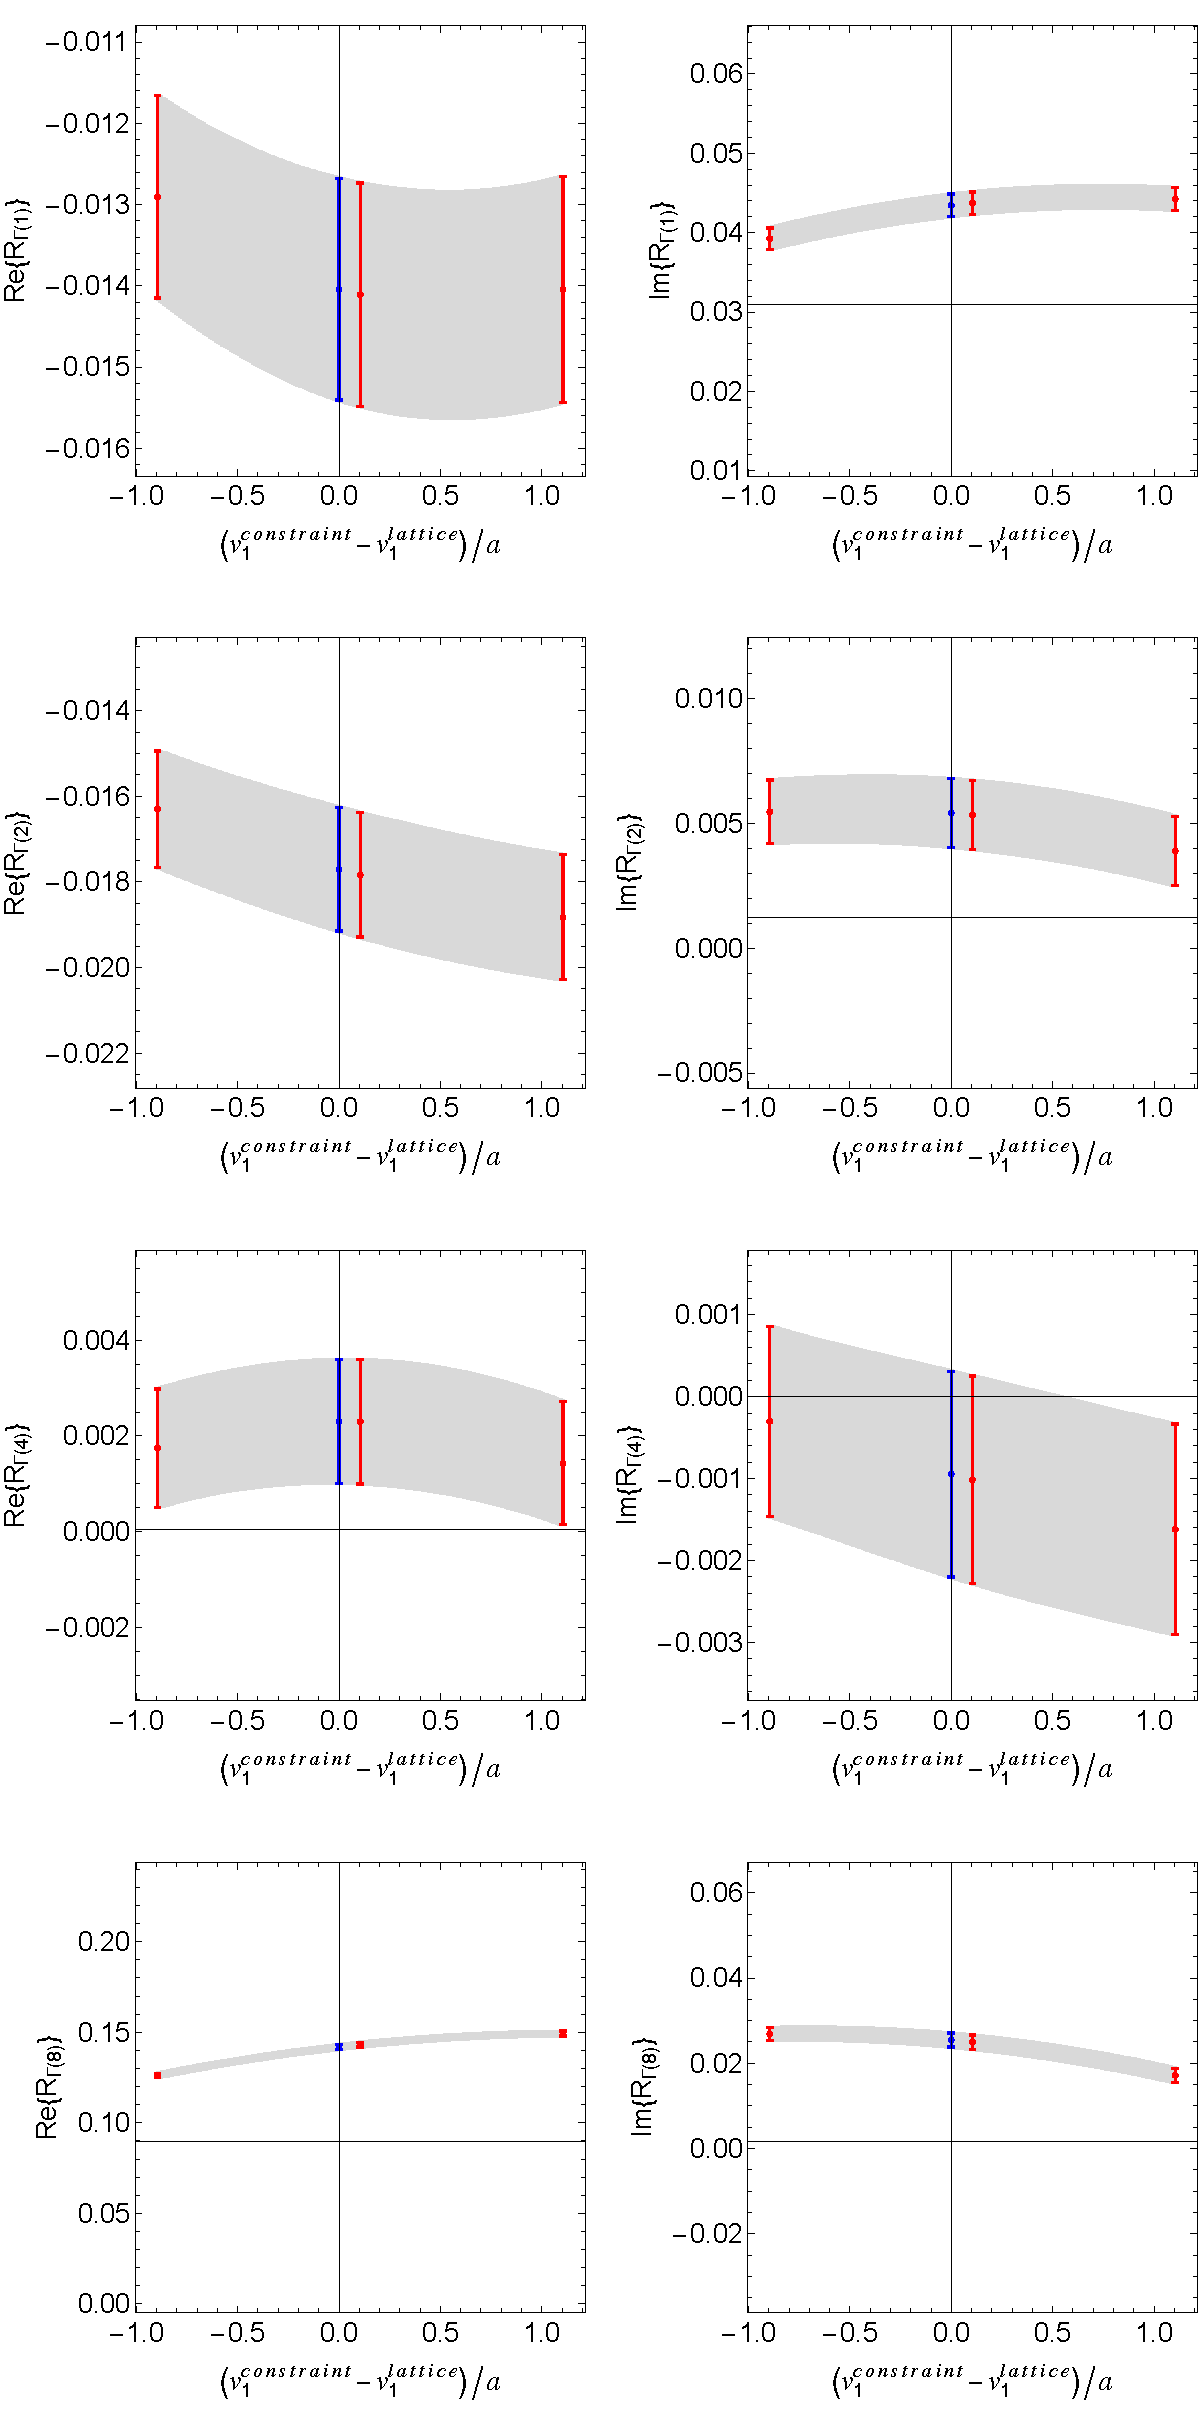
\includegraphics[width=0.6\linewidth,height=0.65\textheight,keepaspectratio]{figures/Interpolation_Ex_b120_eta7_P-1.pdf}
    \caption{Quadratic interpolation of the real and imaginary parts of the correlation function for $\vect{b}=\{1,2,0\}$, $\eta=7$, and $\vect{P}\cdot a\hat{L}/(2\pi)=(-1,0,0)$. Red markers indicate the path-averaged lattice data points as a function of their deviation from the ideal constraint trajectory, $\Delta v_1 = (v_1^{\text{constraint}} - v_1^{\text{lattice}})/a$. The gray curve indicates the quadratic interpolant, and the central blue marker represents the final extracted value at $\Delta v_1 = 0$, lying exactly on the required off-axis spatial trajectory.}
    \label{fig:interpolation_ex}
\end{figure}

\subsection{Quark separation vectors and amplitude parity}
\label{sec:b_separation_paths}
In addition to the staple vector $\vect{v}$, the correlation function depends on the spatial separation $\vect{b}$ between the initial and final quark fields. Recall that the real and imaginary parts of the invariant amplitudes ($\tAmp_{iB}^{\text{Re}}$ and $\tAmp_{iB}^{\text{Im}}$) are even and odd functions of the invariant dot product $b \cdot P$, respectively. 

Because the nucleon momentum in our lattice setup is fixed along the $\hat{x_{1}}$-axis ($P = P_1 \hat{x_{1}}$), the longitudinal separation is directly proportional to the $\hat{x_{1}}$-component of the separation vector: $b \cdot P = -P_1 b_1$. Therefore, to isolate the real and imaginary parts of the amplitudes, we must evaluate the correlator at both positive and negative values of $b_1$. By taking the symmetric (even) and antisymmetric (odd) linear combinations of the correlators evaluated at $+b_1$ and $-b_1$, we project out the real and imaginary amplitudes required for the $x$-dependent Fourier transform. The numerical Fourier transform over $b \cdot P$ requires a wide and dense grid of the separation vector $\vect{b}$. Figures \ref{fig:bL_bT_path}-\ref{fig:bL_bT_standard} show the parameter space of our calculations. The left panel shows the discrete Cartesian grid in the $b_1-b_2$ plane. The right panel shows how this grid maps onto the phenomenologically relevant invariant Variable Space spanned by $(b \cdot P)\hat{L}/(2\pi)$ and the absolute separation $|b|/a$; the mapping shifts with the target Collins-Soper parameter $\hat{\zeta}$. Where, $\hat{L}$ is the spatial lattice length $\hat{L}=32$, and $a=0.11403\text{ fm}$ is the lattice spacing. 

\begin{figure}[htpb]
    \centering
    \begin{minipage}{0.35\textwidth}
        \centering
        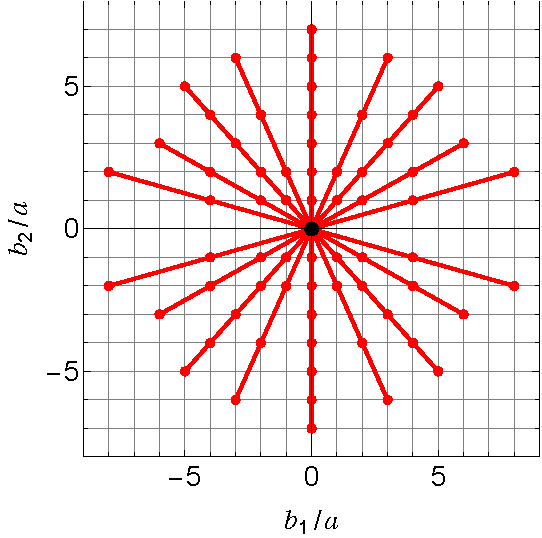
\includegraphics[width=\linewidth]{figures/bL_bT_plot.pdf}
        \caption{The sampled operator separation vectors mapped in the spatial $b_1-b_2$ plane (where $b_1 \equiv b_L$ and $b_2 \equiv b_T$).}
        \label{fig:bL_bT_path}
    \end{minipage}
    \hspace{0.05\textwidth} % Adds a controlled gap between the two smaller images
    \begin{minipage}{0.45\textwidth}
        \centering
        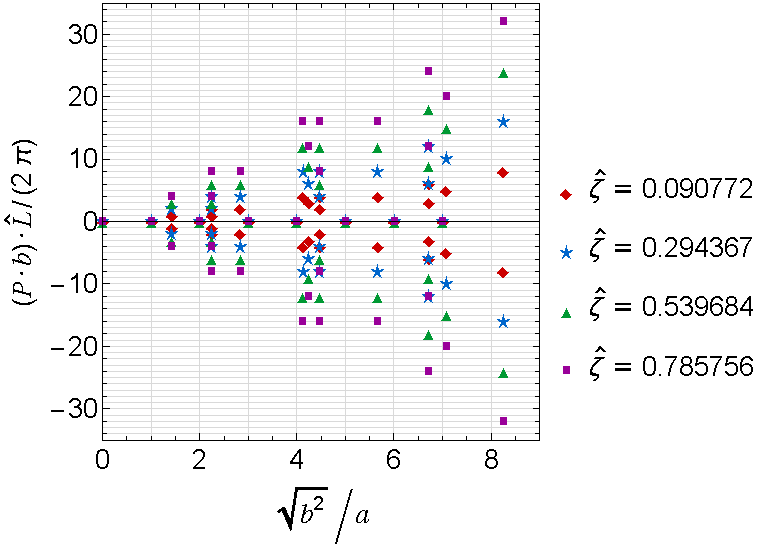
\includegraphics[width=\linewidth]{figures/Pb_bsq_plot.pdf}
        \caption{Mapping of the spatial lattice vectors into the physical invariant Variable Space $(b \cdot P/(2\pi), |b|/a)$. The trajectories diverge based on the selected target $\hat{\zeta}$.}
        \label{fig:bL_bT_standard}
    \end{minipage}
\end{figure}
The gauge-link paths used to reach each $\vect{b}$ and their path averaging are listed in Appendix~\ref{app:paths}.

\subsection{Solving for the real and imaginary amplitudes}
\label{sec:solving_amplitudes}
We contract the amplitude decomposition of Eq.~\eqref{eq-phitildedecomp} with the lattice kinematics $P^\mu=(E_N,-|\vec P^1|,0,0)$, $b^\mu=(0,b_1,b_2,0)$, $v^\mu=\pm n^\prime(0,v_1,0,v_3)$ and $S^\mu=(0,0,0,1)$ for each of $\gamma^0,\ldots,\gamma^3$. Throughout this derivation, $\bvec^1$ and $\bvec^2$ denote the contravariant components of $\bvec$, so that $\bvec^1=b_L$ and $\bvec^2=b_T$ in this frame. The invariant dot product is $\bvec\cdot\bvec$; it is the quantity written $\bvec^2$ in the arguments of the amplitudes $\tAmp_i(\bvec^2,\ldots)$ and is never a component. $R_{\Gamma}$ denotes the lattice ratio observable associated with the Dirac structure $\Gamma$, normalized so that $\widetilde\Phi^{[\Gamma]}_\unsub=E_N R_\Gamma$. % TODO(Hari): define R_Gamma here from the thesis three-point/two-point ratio (thesis Sec. 3.7)
The index $i\in\{1,2,4,8\}$ in $R_{\Gamma(i)}$ labels the Dirac structure by the bit-encoded convention $\Gamma(n)=\gamma_1^{n_0}\gamma_2^{n_1}\gamma_3^{n_2}\gamma_4^{n_3}$, with $\Gamma(1)=[+i\gamma^1]$, $\Gamma(2)=[-i\gamma^2]$, $\Gamma(4)=[+i\gamma^3]$ and $\Gamma(8)=[\gamma^0]$. Taking the symmetric and antisymmetric combinations of the data at $+b^1$ and $-b^1$ projects out the $b^1$-even (real) and $b^1$-odd (imaginary) amplitudes. The full algebra is in Appendix~\ref{app:solve}. The results are
Recalling that $v \tcdot P = v_1 P^1 = v^1 |P^1|$ in our chosen frame, each amplitude structure has its own conversion factor. Applying this mapping to the real components yields the final accessible amplitudes on the lattice:
\begin{widetext}
\begin{align}
    \Aboxed{\tAmp^{\text{Re}}_2 = & \frac{1}{2}\text{Re}\{ R_{\Gamma(8)}\}^{[b^{1}\text{-even}]} }\\
    \Aboxed{\tBmp^{\text{Re}}_1 = & \frac{E_{N}|P^1|v^1}{2\mN^2  v^3} \text{Im}\{ R_{\Gamma(4)}\}^{[b^{1}\text{-even}]}}\\
    \Aboxed{\tAmp^{\text{Re}}_{12}=&\frac{-1}{2\mN  \bvec^2}\left[\text{Re}\{ R_{\Gamma(1)}\}^{[b^{1}\text{-even}]}+\frac{v^3}{v^1}\text{Re}\{ R_{\Gamma(4)}\}^{[b^{1}\text{-even}]}\right]}\\
    \Aboxed{\tBmp^{\text{Re}}_8=&\frac{-E_N |P^1|}{ 2\mN^3 \bvec^2 }\left[\text{Im}\{ R_{\Gamma(8)}\}^{[b^{1}\text{-even}]}+\frac{|\vec{P}^1|v^3}{E_N v^1}\text{Re}\{ R_{\Gamma(4)}\}^{[b^{1}\text{-even}]}+ 2\mN  \frac{|\vec{P}^1|}{E_N} \bvec^2  \tAmp^{\text{Re}}_{12}\right]}
\end{align}
\end{widetext}
Applying the same scaling factors to the imaginary counterparts provides the complementary $b$-odd contributions:
\begin{widetext}
\begin{align}
    \Aboxed{\tAmp^{\text{Im}}_2 = & \frac{1}{2}\text{Im}\{ R_{\Gamma(8)}\}^{[b^{1}\text{-odd}]} }\\
    \Aboxed{\tBmp^{\text{Im}}_1 = & \frac{-E_{N}|P^1|v^1}{2\mN^2 v^3} \text{Re}\{ R_{\Gamma(4)}\}^{[b^{1}\text{-odd}]}}\\
    \Aboxed{\tAmp^{\text{Im}}_{12}=&\frac{-1}{2\mN  \bvec^2}\left[\text{Im}\{ R_{\Gamma(1)}\}^{[b^{1}\text{-odd}]}+\frac{v^3}{v^1}\text{Im}\{ R_{\Gamma(4)}\}^{[b^{1}\text{-odd}]}\right]}\\
     \Aboxed{\tBmp^{\text{Im}}_8=&\frac{E_N|P^1|}{ 2\mN^3 \bvec^2  }\left[\text{Re}\{ R_{\Gamma(8)}\}^{[b^{1}\text{-odd}]}-\frac{|\vec{P}^1|v^3}{E_N v^1}\text{Im}\{ R_{\Gamma(4)}\}^{[b^{1}\text{-odd}]}- 2\mN  \frac{|\vec{P}^1|}{E_N} \bvec^2  \tAmp^{\text{Im}}_{12}\right]}
\end{align}
\end{widetext}

\subsection{Constructing the amplitudes \texorpdfstring{$\tAmp_{2B}$}{A2B} and \texorpdfstring{$\tAmp_{12B}$}{A12B}}
\label{sec:effective_amplitudes}

With the invariant amplitudes isolated by parity projection, we now combine them into the amplitudes $\tAmp_{2B}$ and $\tAmp_{12B}$ of Eq.~\eqref{eq-ABamps_sivers}, with $R(\zetahat^2)$ from Eq.~\eqref{eq-lindeprel}. 
To apply these expressions in our simulated lattice geometry, we map the contravariant spatial indices to our physical grid parameters. We define the longitudinal spatial separation as $b_L \equiv b^1$ and the transverse spatial separation as $b_T \equiv b^2$.
The invariant $\bvec\cdot\bvec$ then expands to $b_L^2 + b_T^2$ and enters only through the arguments of the amplitudes, while the prefactors in the $\tAmp_{12}$ and $\tBmp_8$ expressions below depend on the component $b_T=\bvec^2$ alone. We identify the longitudinal nucleon momentum as $P_L \equiv P^1$. 

We begin with the defining linear combination for the unpolarized amplitude, $\tAmp_{2B}$. Splitting this amplitude into its real and imaginary components yields:
\begin{align}
    \tAmp_{2B}^{\text{Re}}(b_L, b_T, \hat{\zeta}) &= \tAmp_2^{\text{Re}} + R(\zetahat^2) \tBmp_1^{\text{Re}} \\
    \tAmp_{2B}^{\text{Im}}(b_L, b_T, \hat{\zeta}) &= \tAmp_2^{\text{Im}} + R(\zetahat^2) \tBmp_1^{\text{Im}}
\end{align}

Substituting the parity-projected lattice ratio observables of Sec.~\ref{sec:solving_amplitudes} (and applying our $b_L, P_L$ geometric mapping), we obtain the real part of $\tAmp_{2B}$ as an expression computable directly from our grid coordinates:
\begin{widetext}
\begin{align}
    \tAmp_{2B}^{\text{Re}}(b_L, b_T, \hat{\zeta}) &= \frac{1}{2}\text{Re}\{ R_{\Gamma(8)}\}^{[b_L\text{-even}]} + R(\zetahat^2) \frac{E_{N}|P_L|v^1}{2\mN^2 v^3} \text{Im}\{ R_{\Gamma(4)}\}^{[b_L\text{-even}]}
\end{align}
\end{widetext}

The same substitution for the imaginary component, now with the $b_L$-odd projected data sets so that time-reversal parity is preserved, gives:
\begin{widetext}
\begin{align}
    \tAmp_{2B}^{\text{Im}}(b_L, b_T, \hat{\zeta}) &= \frac{1}{2}\text{Im}\{ R_{\Gamma(8)}\}^{[b_L\text{-odd}]} - R(\zetahat^2) \frac{E_{N}|P_L|v^1}{2\mN^2 v^3} \text{Re}\{ R_{\Gamma(4)}\}^{[b_L\text{-odd}]}
\end{align}
\end{widetext}

The amplitude that drives the Sivers shift, $\tAmp_{12B}$, combines the structures $\tAmp_{12}$ and $\tBmp_8$. Its real and imaginary decompositions are defined as:
\begin{align}
    \tAmp_{12B}^{\text{Re}}(b_L, b_T, \hat{\zeta}) &= \tAmp_{12}^{\text{Re}} - R(\zetahat^2) \tBmp_8^{\text{Re}} \\
    \tAmp_{12B}^{\text{Im}}(b_L, b_T, \hat{\zeta}) &= \tAmp_{12}^{\text{Im}} - R(\zetahat^2) \tBmp_8^{\text{Im}}
\end{align}

Because the terms within $\tAmp_{12B}$ are more complex, we first write out the inner constituent $\tAmp_{12}^{\text{Re}}$ in terms of the grid parameters $b_L$ and $b_T$. The real part of the leading-twist term becomes:
\begin{align}
    \tAmp^{\text{Re}}_{12} &= \frac{-1}{2\mN\, b_T} \left[\text{Re}\{ R_{\Gamma(1)}\}^{[b_L\text{-even}]} + \frac{v^3}{v^1}\text{Re}\{ R_{\Gamma(4)}\}^{[b_L\text{-even}]}\right]
\end{align}

Substituting this internal structure alongside the expansion for $\tBmp_8^{\text{Re}}$ gives the full equation for the real part entering the Sivers integration:
\begin{widetext}
\begin{align}
    \tAmp_{12B}^{\text{Re}}(b_L, b_T, \hat{\zeta}) &= \tAmp^{\text{Re}}_{12} - R(\zetahat^2) \Bigg( \frac{-E_N |P_L|}{ 2\mN^3\, b_T }\Bigg[\text{Im}\{ R_{\Gamma(8)}\}^{[b_L\text{-even}]} + \frac{|P_L|v^3}{E_N v^1}\text{Re}\{ R_{\Gamma(4)}\}^{[b_L\text{-even}]} \nonumber \\
    & \qquad + 2\mN  \frac{|P_L|}{E_N}\, b_T\,  \tAmp^{\text{Re}}_{12}\Bigg] \Bigg)
\end{align}
\end{widetext}

Following the same procedure for the imaginary (T-odd) components, we first define the internal $b_L$-odd constituent $\tAmp^{\text{Im}}_{12}$:
\begin{align}
    \tAmp^{\text{Im}}_{12} &= \frac{-1}{2\mN\, b_T} \left[\text{Im}\{ R_{\Gamma(1)}\}^{[b_L\text{-odd}]} + \frac{v^3}{v^1}\text{Im}\{ R_{\Gamma(4)}\}^{[b_L\text{-odd}]}\right]
\end{align}

We then insert it to obtain the full equation for the imaginary part of the Sivers amplitude:
\begin{widetext}
\begin{align}
    \tAmp_{12B}^{\text{Im}}(b_L, b_T, \hat{\zeta}) &= \tAmp^{\text{Im}}_{12} - R(\zetahat^2) \Bigg( \frac{E_N |P_L|}{ 2\mN^3\, b_T }\Bigg[\text{Re}\{ R_{\Gamma(8)}\}^{[b_L\text{-odd}]} - \frac{|P_L|v^3}{E_N v^1}\text{Im}\{ R_{\Gamma(4)}\}^{[b_L\text{-odd}]} \nonumber \\
    & \qquad - 2\mN  \frac{|P_L|}{E_N}\, b_T\,  \tAmp^{\text{Im}}_{12}\Bigg] \Bigg)
\end{align}
\end{widetext}

\subsection{Mapping to Lorentz-invariant variables}
\label{sec:lorentz_mapping}
At this stage, the amplitudes $\tAmp_{2B}$ and $\tAmp_{12B}$ are discrete functions of the Cartesian lattice grid parameters $b_L$ and $b_T$. Extracting the dependence on the longitudinal momentum fraction $x$, however, requires the Fourier transform over the Lorentz-invariant inner product $P \cdot b$. To perform this integration, we first show that our simulated Cartesian lattice coordinates map one-to-one to the invariant Variable Space.

In our selected kinematic frame, the 4-vectors for the nucleon momentum and spatial separation are defined as:
\begin{align}
    P^{\mu} &= (E_N, P_L, 0, 0) \\
    b^{\mu} &= (0, b_L, b_T, 0)
\end{align}

Evaluating the inner product using the Minkowski metric signature $(+,-,-,-)$, the temporal and transverse orthogonal components vanish, leaving:
\begin{align}
    P \cdot b &= P_0 b^0 - P_1 b^1 - P_2 b^2 - P_3 b^3 \nonumber \\
              &= - P_L b_L \label{eq:pb_minus_pl_bl}
\end{align}

Inverting this identity expresses the longitudinal Cartesian lattice coordinate $b_L$ as a continuous function of the invariant scalar $P \cdot b$ and the fixed lattice momentum $P_L$:
\begin{align}
    b_L &= \frac{P \cdot b}{-P_L}
\end{align}

To complete the geometric mapping, we must also express the invariant $\bvec\cdot\bvec=b_L^2+b_T^2$, the argument written $\bvec^2$ in the amplitudes, through $P\cdot b$. The prefactors in the $\tAmp_{12}$ and $\tBmp_8$ expressions depend only on $b_T$, which is independent of $P\cdot b$. Substituting our Lorentz expression for $b_L$ into $\bvec\cdot\bvec$ yields:
\begin{align}
    \bvec^2 &= \left( \frac{P \cdot b}{-P_L} \right)^2 + b_T^2
\end{align}

By replacing $b_L$ and $\bvec^2$ with these invariant expressions, we transform our discrete lattice amplitudes into continuous functions of the Lorentz-invariant variables:
\begin{align}
    \tAmp_{iB}(b_L, b_T, \hat{\zeta}) \quad \xrightarrow{\text{Coordinate Transformation}} \quad \tAmp_{iB}\left( P \cdot b, \bvec^2, \hat{\zeta} \right)
\end{align}

With the amplitudes now expressed as functions of $P \cdot b$, the Fourier transform of Eq.~\eqref{eq:sivers_shift_xdep} can be evaluated directly. This connects the Euclidean correlation ratios evaluated on the lattice to the physical, $x$-dependent phenomenological observables needed to study the Sivers effect.

\subsection{Parity checks and the extracted amplitudes}
\label{sec:numerical_amplitudes}
Before examining the lattice data across the different Collins-Soper scales ($\hat{\zeta}$), we check the parity constraints of Eq.~\eqref{eq-ReIm-parity}. Since $P\cdot b=-P_Lb_L$ (Eq.~\eqref{eq:pb_minus_pl_bl}), the real amplitudes $\tAmp_{2B}^{\text{Re}}$ and $\tAmp_{12B}^{\text{Re}}$ must be even in the Cartesian longitudinal separation $b_L$, and the imaginary amplitudes $\tAmp_{2B}^{\text{Im}}$ and $\tAmp_{12B}^{\text{Im}}$ must be odd. The lattice data in the figures below show these even and odd profiles along the $b_L$ axis. % TODO(Hari): the profiles follow from the projection by construction; add the size of the opposite-parity part as an actual check

However, the statistical quality of the extracted signals differs between amplitudes. While the unpolarized amplitudes ($\tAmp_{2B}^{\text{Re}}$ and $\tAmp_{2B}^{\text{Im}}$) and the real Sivers amplitude ($\tAmp_{12B}^{\text{Re}}$) show clear, statistically resolvable signals across the simulated data, the imaginary Sivers amplitude ($\tAmp_{12B}^{\text{Im}}$) does not. Across all evaluated nucleon momenta and staple extents, the extracted lattice data for $\tAmp_{12B}^{\text{Im}}$ is dominated by gauge noise and is statistically compatible with zero. We cannot constrain a model for this component. We therefore neglect $\tAmp_{12B}^{\text{Im}}$ from further analysis: we drop the $\sin(x(b\cdot P))\tAmp_{12B}^{\text{Im}}$ term in Eq.~\eqref{eq:sivers_shift_xdep} and evaluate the $x$-dependent Sivers shift using only the $\tAmp_{12B}^{\text{Re}}$ data. % TODO(Hari): this is an approximation; estimate its effect on the shift and list it as a systematic

Figures~\ref{fig:amps_P1} and~\ref{fig:amps_P4} show the extracted amplitudes at the smallest and largest simulated momenta; Figs.~\ref{fig:amps_P2} and~\ref{fig:amps_P3} in Appendix~\ref{app:amps} show the other two.
\begin{figure*}[htbp]
\centering
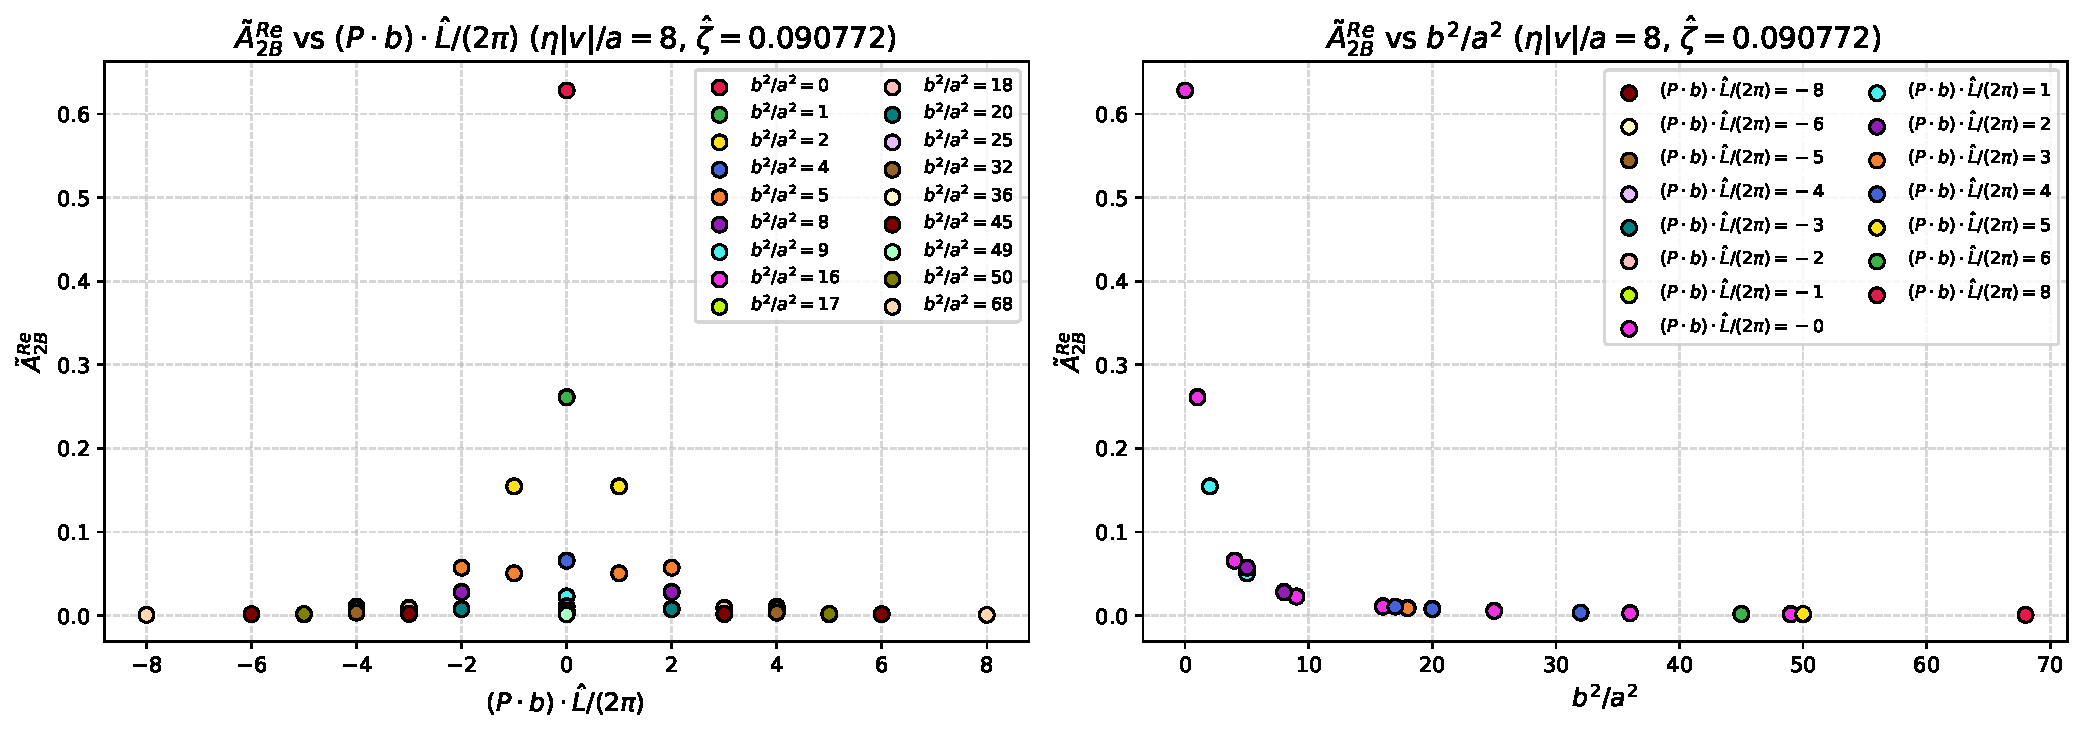
\includegraphics[width=0.48\linewidth]{figures/amps/ReA2B_Pb_bsq_eta8_PL-1_2D.pdf}\hfill
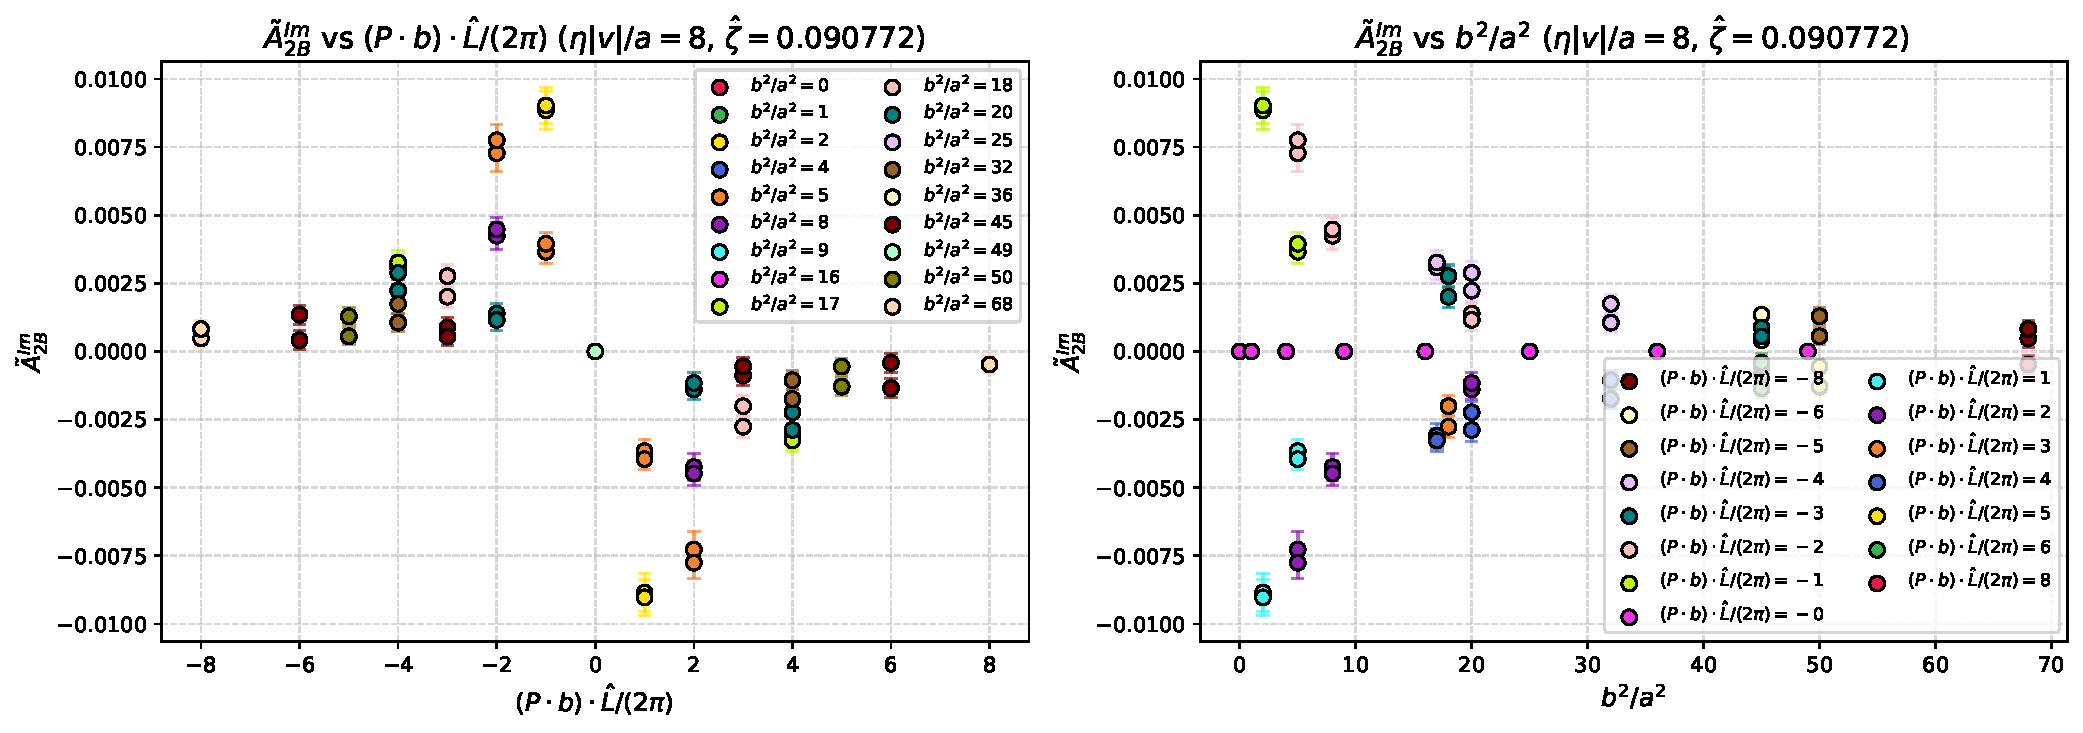
\includegraphics[width=0.48\linewidth]{figures/amps/ImA2B_Pb_bsq_eta8_PL-1_2D.pdf}\\[1ex]
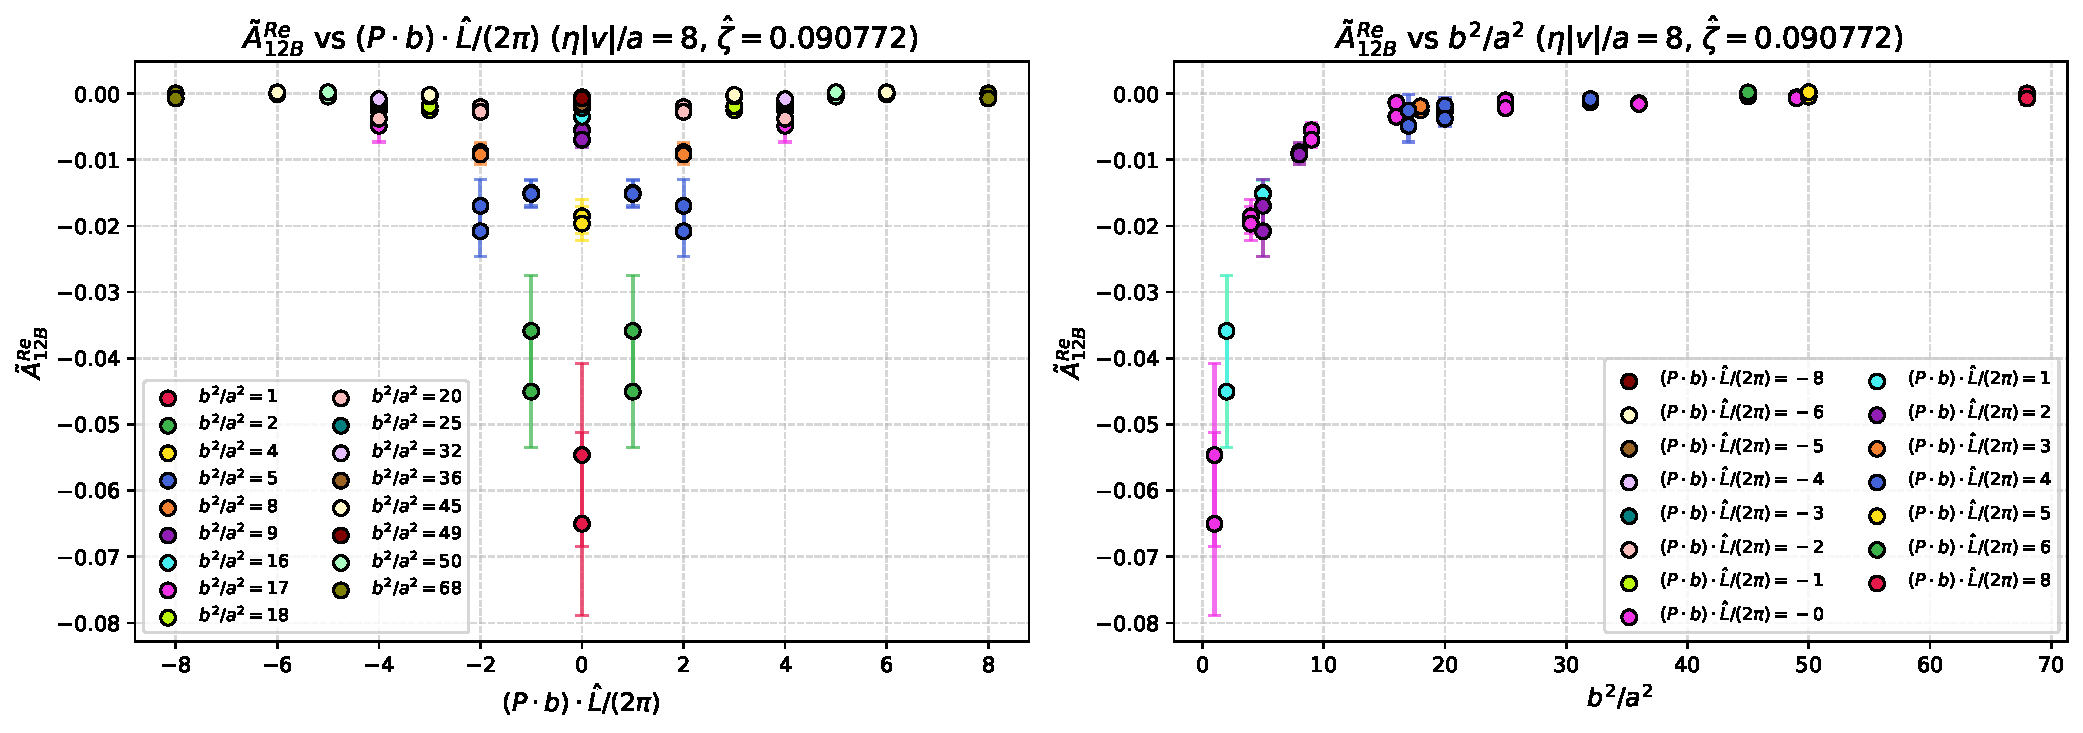
\includegraphics[width=0.48\linewidth]{figures/amps/ReA12B_Pb_bsq_eta8_PL-1_2D.pdf}\hfill
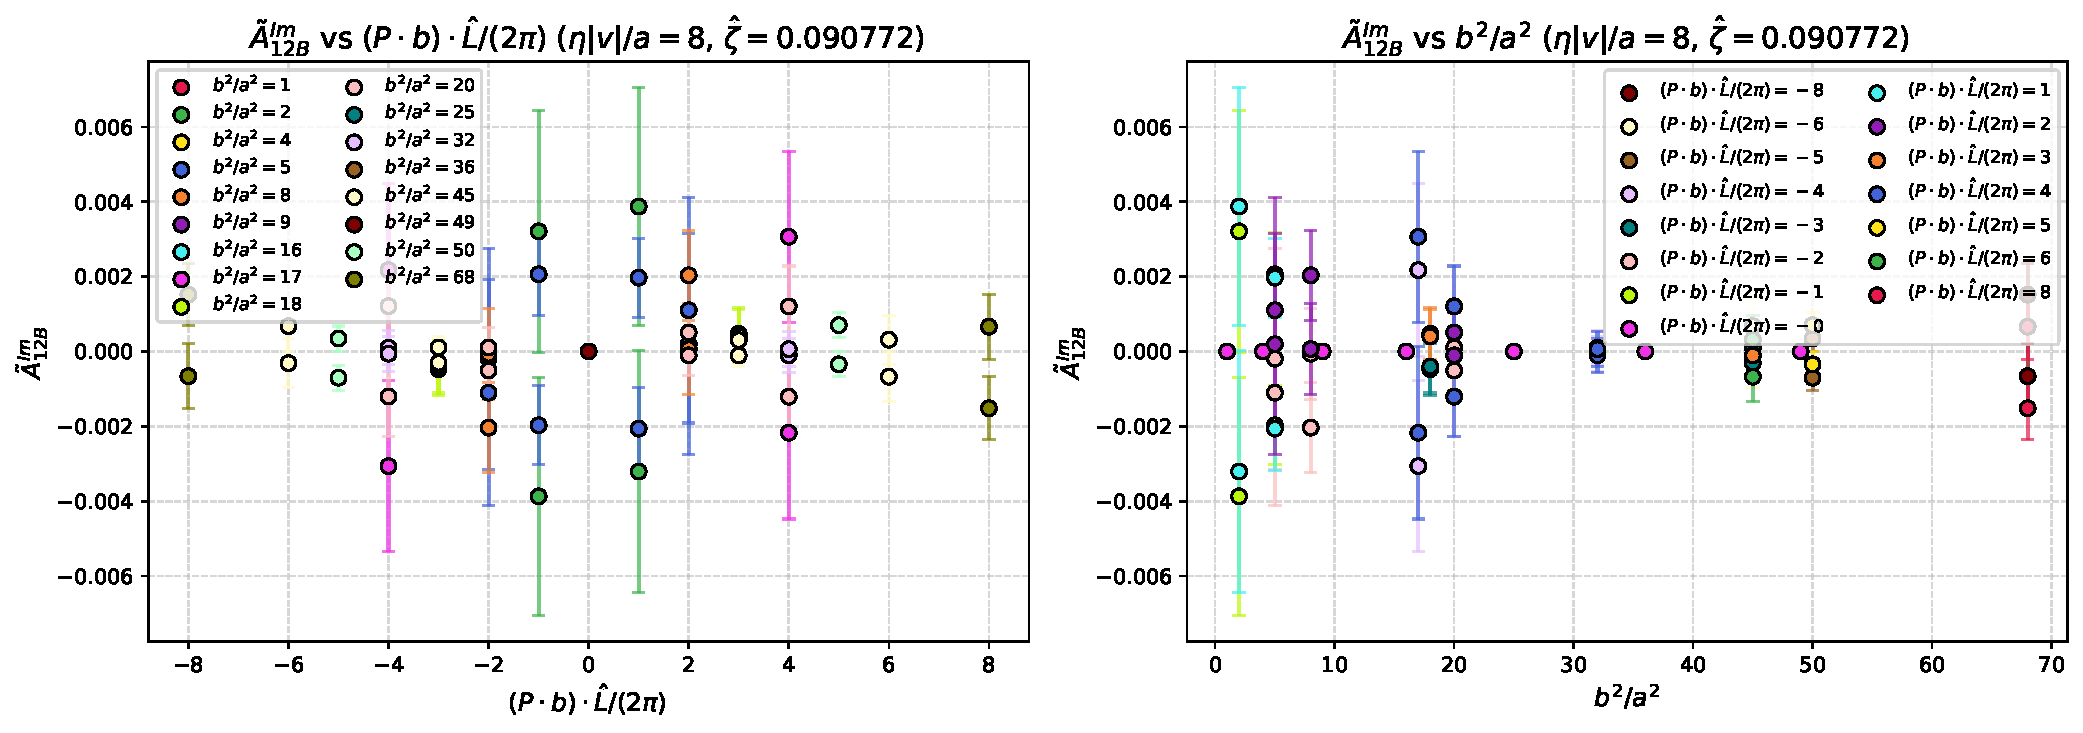
\includegraphics[width=0.48\linewidth]{figures/amps/ImA12B_Pb_bsq_eta8_PL-1_2D.pdf}
\caption{Real (left) and imaginary (right) parts of $\tAmp_{2B}$ (top) and $\tAmp_{12B}$ (bottom) in the $((\vect{P}\cdot\vect{b})\hat{L}/(2\pi),\,b^2/a^2)$ space at fixed $\eta|\vect{v}|/a=8$, for $\vect{P}\cdot a\hat{L}/(2\pi)=(-1,0,0)$ ($\hat\zeta=0.090772$). No signal is discernible in $\tAmp_{12B}^{\text{Im}}$.}
\label{fig:amps_P1}
\end{figure*}

\begin{figure*}[htbp]
\centering
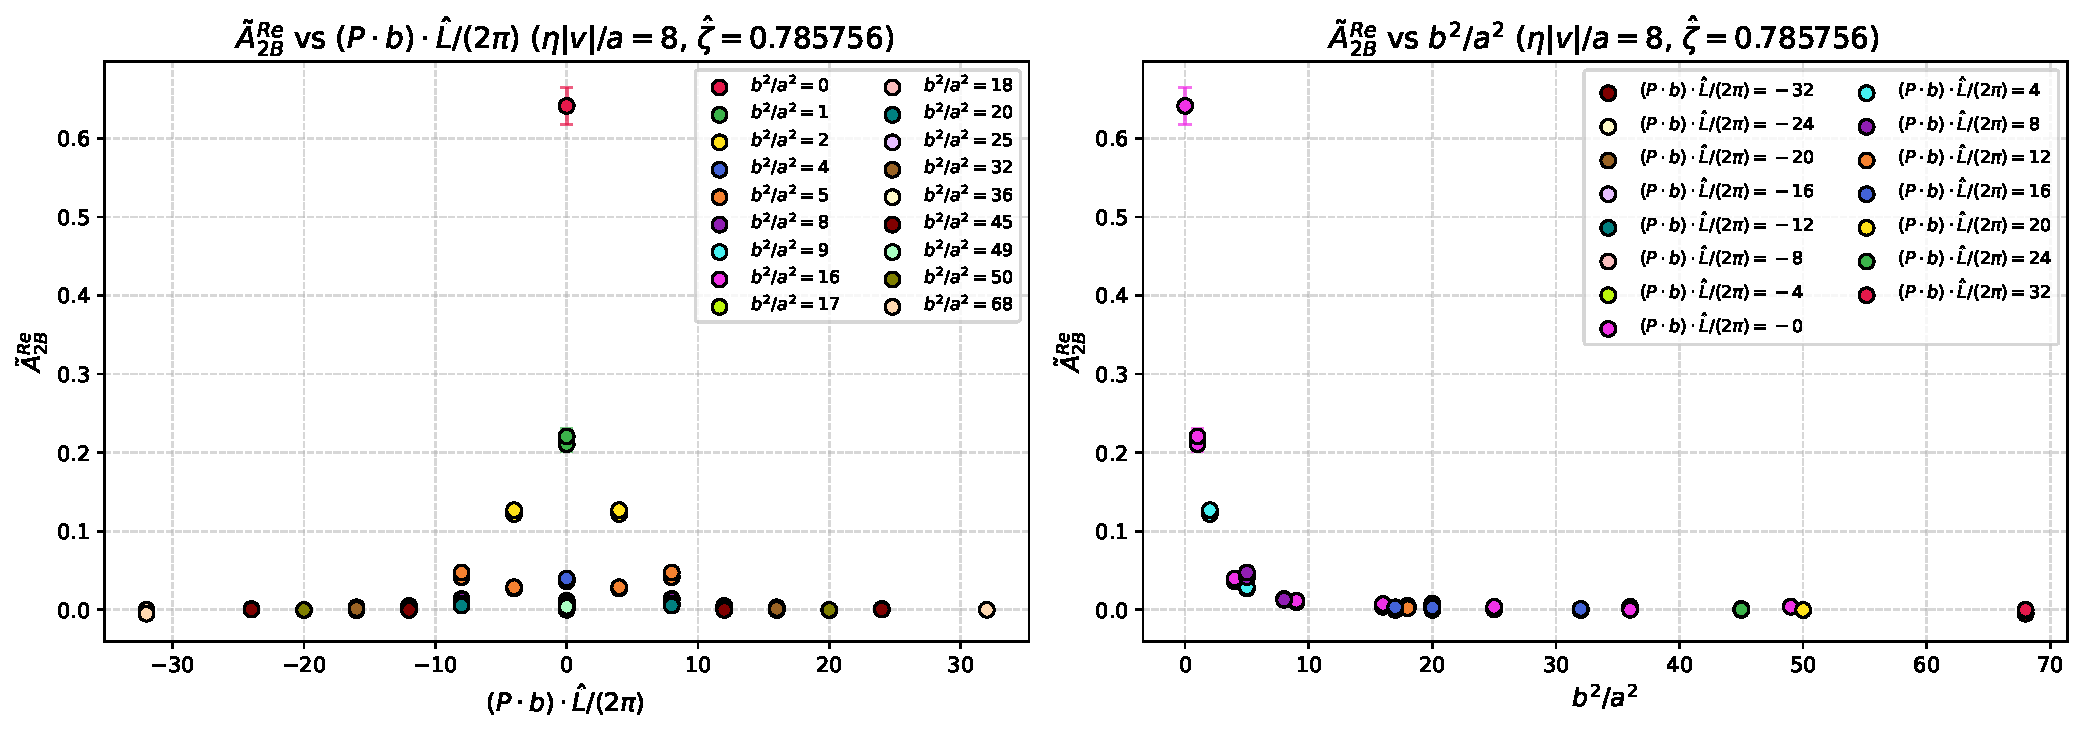
\includegraphics[width=0.48\linewidth]{figures/amps/ReA2B_Pb_bsq_eta8_PL-4_2D.pdf}\hfill
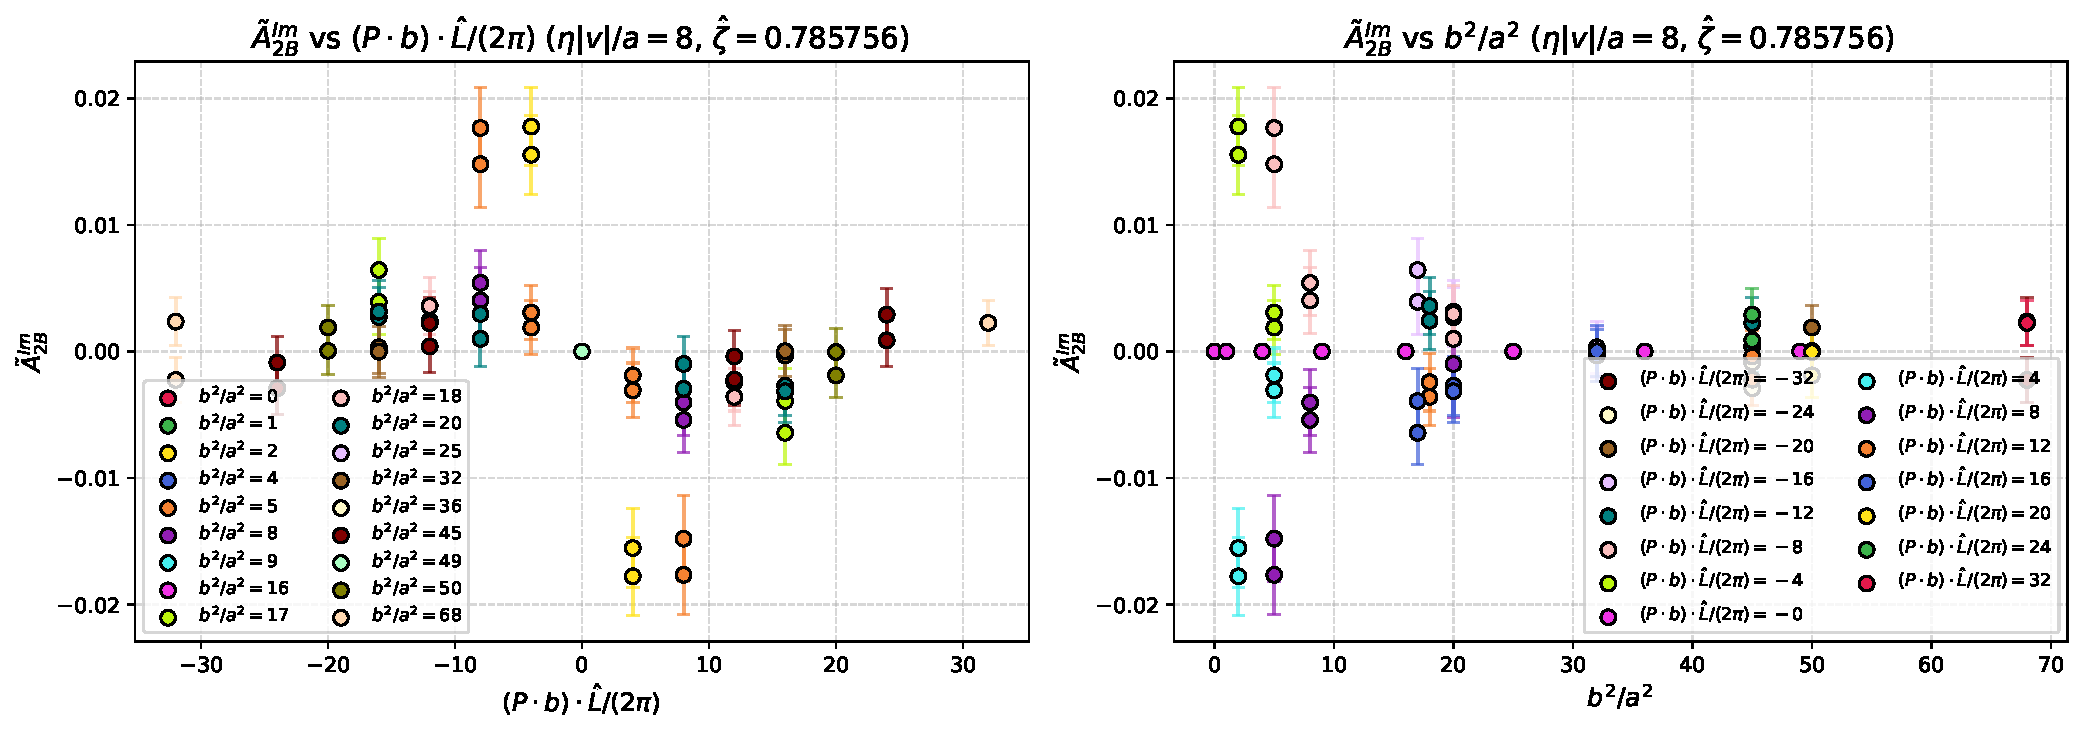
\includegraphics[width=0.48\linewidth]{figures/amps/ImA2B_Pb_bsq_eta8_PL-4_2D.pdf}\\[1ex]
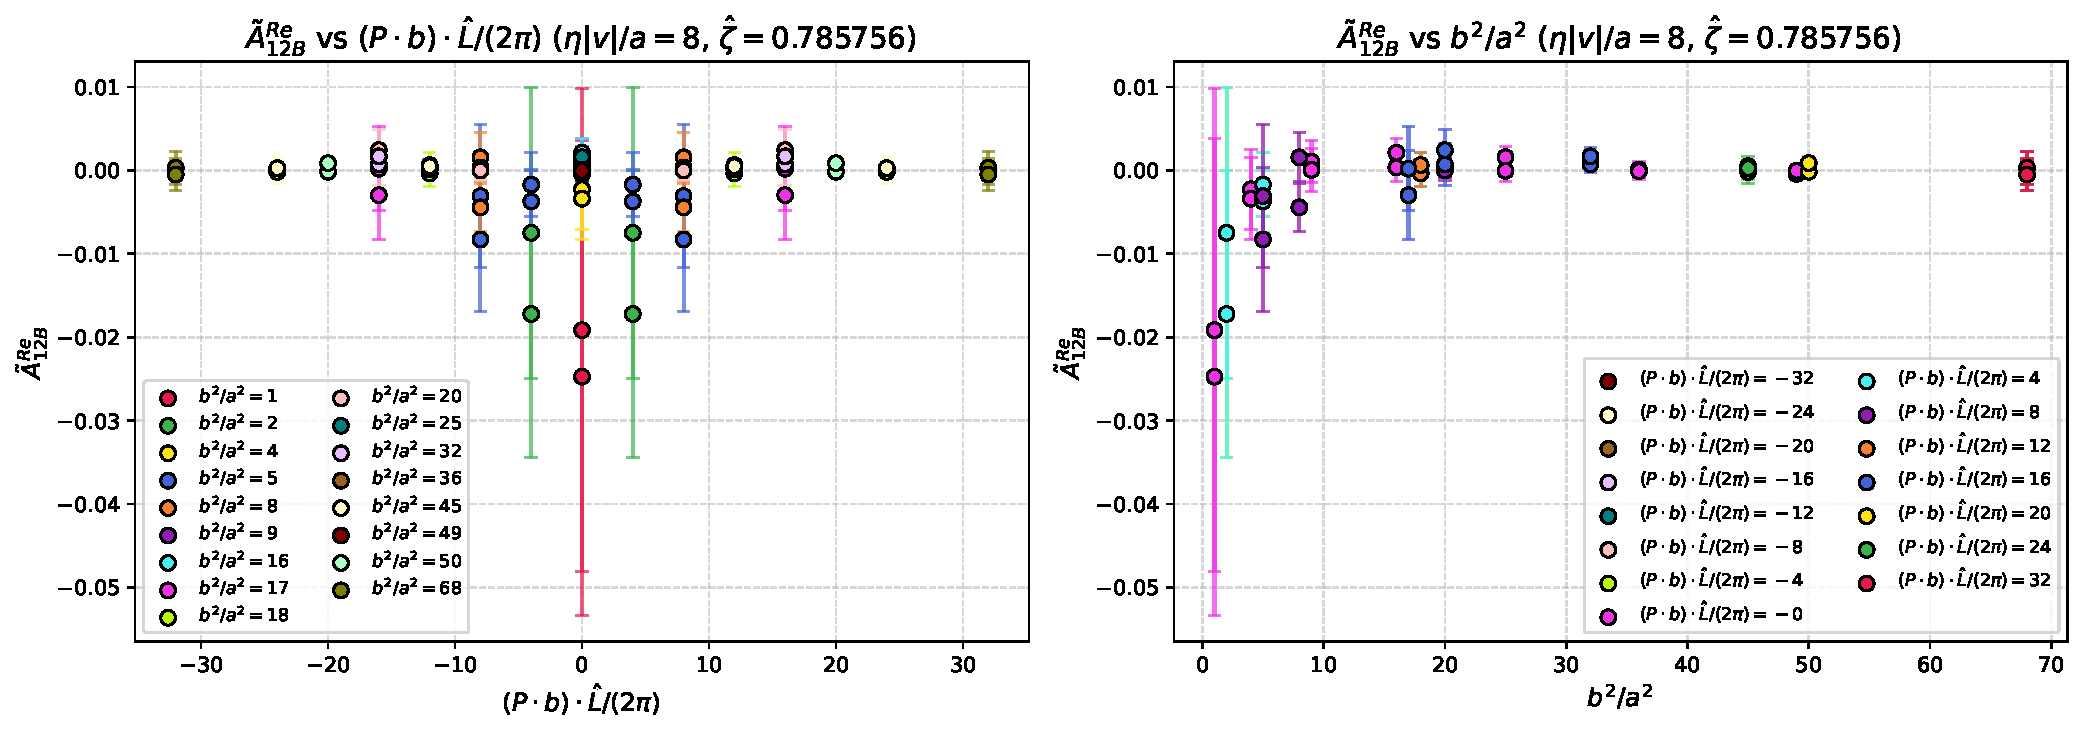
\includegraphics[width=0.48\linewidth]{figures/amps/ReA12B_Pb_bsq_eta8_PL-4_2D.pdf}\hfill
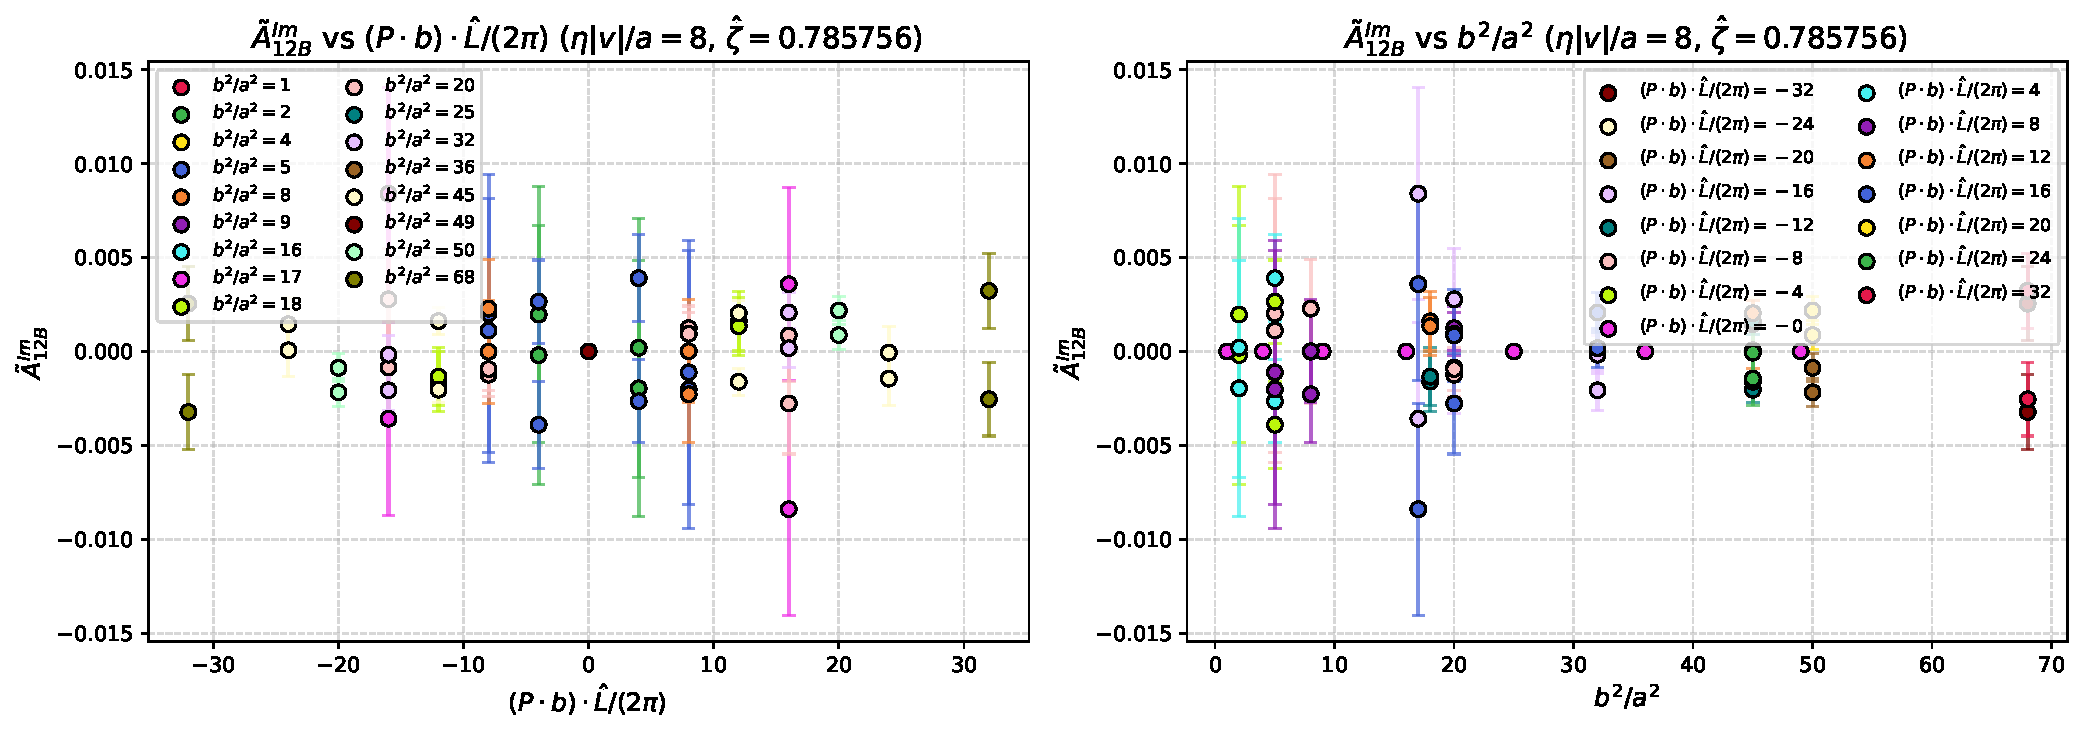
\includegraphics[width=0.48\linewidth]{figures/amps/ImA12B_Pb_bsq_eta8_PL-4_2D.pdf}
\caption{Real (left) and imaginary (right) parts of $\tAmp_{2B}$ (top) and $\tAmp_{12B}$ (bottom) in the $((\vect{P}\cdot\vect{b})\hat{L}/(2\pi),\,b^2/a^2)$ space at fixed $\eta|\vect{v}|/a=8$, for $\vect{P}\cdot a\hat{L}/(2\pi)=(-4,0,0)$ ($\hat\zeta=0.785756$).}
\label{fig:amps_P4}
\end{figure*}


